\begin{figure}[!ht]
    \centering
    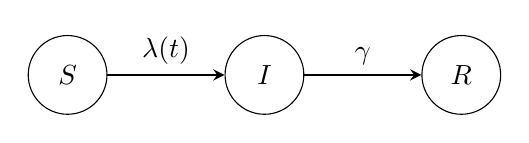
\begin{tikzpicture}[cap=round,>=latex]
    \tikzstyle{comp} = [circle, minimum size=1cm, draw=black, text centered]
    \tikzstyle{compr} = [circle, minimum size=1cm, draw=red, text centered, line width=0.75mm,dashed]
    \tikzstyle{arrow} = [thick,->,>=stealth]
    \tikzstyle{arrowb} = [ultra thick,dotted,->,>=stealth,blue]
    \tikzstyle{arrowg} = [ultra thick,dashed,->,>=stealth,red]
    \node (S) [comp] {$S$};
    \node (I) [comp, right of=S, xshift=1.5cm] {$I$};
    \node (R) [comp, right of=I, xshift=1.5cm] {$R$};
    \draw [arrow] (S) to node[anchor=south] {$\lambda(t)$} (I);
    \draw [arrow] (I) to node[anchor=south] {$\gamma$} (R);
    \end{tikzpicture}
    \caption{Schematic representation of the SIR compartmental model.}
    \label{fig:model}
\end{figure}